\newpage
\noindent \textbf{Dataset}: Online News Popularity Data Set. \\
URL: http://archive.ics.uci.edu/ml/datasets/Online+News+Popularity

\subsection*{Explanation of choice}
This dataset is based on recent articles, published in 2013--2015 years, so the data is actual up to now.   
Moreover, it is composed of different types of variables. 

\subsection*{Data Set Information}

\begin{itemize}
\item The articles were published by Mashable (www.mashable.com) and their content as the rights to reproduce it belongs to them. Hence, this dataset does not share the original content but some statistics associated with it. The original content could be publicly accessed and retrieved using the provided urls.  
\item Acquisition date: January 8, 2015  
\item The estimated relative performance values were estimated by the authors using a Random Forest classifier and a rolling windows as assessment method. See their article for more details on how the relative performance values were set.
\item From initial data-set we chose $34$ attributes and $10000$ instances (instances were chosen randomly).
\end{itemize}


\textbf{Attribute Information}:
\begin{enumerate}
\item \texttt{url}: URL of the article (non-predictive)
\item \texttt{timedelta}: Days between the article publication and the dataset acquisition (non-predictive) 
\item \texttt{n\_tokens\_title}: Number of words in the title 
\item \texttt{n\_tokens\_content}: Number of words in the content
\item \texttt{n\_unique\_tokens}: Rate of unique words in the content
\item \texttt{num\_hrefs}: Number of links 
\item \texttt{num\_self\_hrefs}: Number of links to other articles published by Mashable 
\item \texttt{num\_imgs}: Number of images  
\item \texttt{num\_videos}: Number of videos 
\item \texttt{average\_token\_length}: Average length of the words in the content
\item \texttt{num\_keywords}: Number of keywords in the metadata 
\item  \texttt{data\_channel\_is\_lifestyle}: Is data channel 'Lifestyle'? 
\item \texttt{data\_channel\_is\_entertainment}: Is data channel 'Entertainment'? 
\item \texttt{data\_channel\_is\_bus}: Is data channel 'Business'? 
\item \texttt{data\_channel\_is\_socmed}: Is data channel 'Social Media'? 
\item \texttt{data\_channel\_is\_tech}: Is data channel 'Tech'?  
\item \texttt{data\_channel\_is\_world}: Is data channel 'World'?

\item \texttt{self\_reference\_avg\_sharess}: Avg. shares of referenced articles in Mashable  
\item \texttt{weekday\_is\_monday}: Was the article published on a Monday?
\item \texttt{weekday\_is\_tuesday}: Was the article published on a Tuesday? 
\item \texttt{weekday\_is\_wednesday}: Was the article published on a Wednesday?
\item \texttt{weekday\_is\_thursday}: Was the article published on a Thursday? 
\item \texttt{weekday\_is\_friday}: Was the article published on a Friday?
\item \texttt{weekday\_is\_saturday}: Was the article published on a Saturday? 
\item \texttt{weekday\_is\_sunday}: Was the article published on a Sunday?
\item \texttt{global\_sentiment\_polarity}:     Text sentiment polarity
\item \texttt{global\_rate\_positive\_words}:    Rate of positive words in the content
\item \texttt{global\_rate\_negative\_words}:    Rate of negative words in the content
\item \texttt{rate\_positive\_words}:           Rate of positive words among non-neutral
\item \texttt{avg\_positive\_polarity}:         Avg. polarity of positive words
\item \texttt{avg\_negative\_polarity}:         Avg. polarity of negative  words 
\item \texttt{title\_sentiment\_polarity}:      Title polarity
\item \texttt{shares}:                        Number of shares (target)
\end{enumerate} 

\section{Assignment 1}
In the first task we consider the attribute called \texttt{shares},  which is the number of article shares in various social networks. Let construct a histogram and boxplot of chosen attribute (see Figure \ref{img:hist_boxplot_shares}). From the histogram wee can see, that the choosen attribute probably has a lognormal distribution, so we construct a new feautre \texttt{$\log$(shares)}. Histogram and boxplot for this new feature \texttt{$\log$(shares)} are presented on  Figure \ref{img:hist_boxplot_log_shares}. 


 
\begin{figure}[h!]
 \begin{center}
    \center 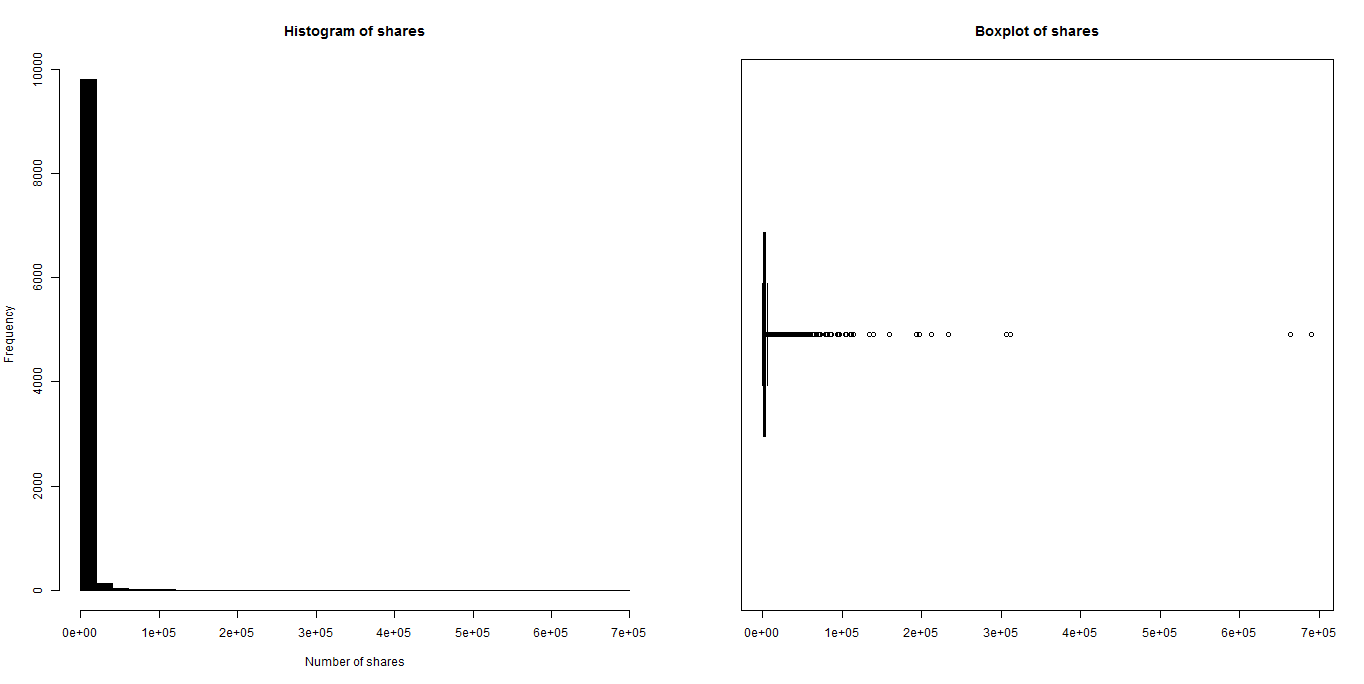
\includegraphics[width = 0.8\textwidth]{hist_boxplot_shares.png}
   \caption{}
   \label{img:hist_boxplot_shares}
 \end{center}
\end{figure} 
\begin{figure}[h!]
 \begin{center}
    \center 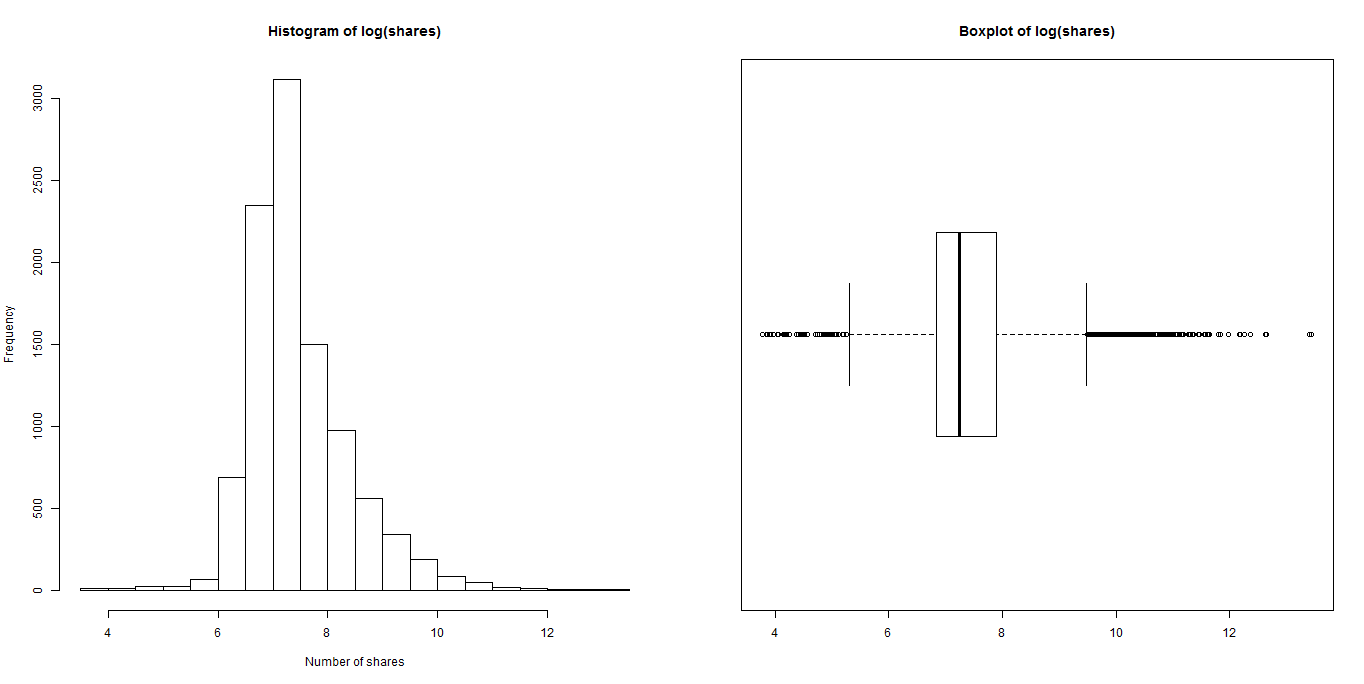
\includegraphics[width = 0.8\textwidth]{hist_boxplot_log_shares.png}
   \caption{}
   \label{img:hist_boxplot_log_shares}
 \end{center}
\end{figure}  

Below we will apply methods to the feature \texttt{$\log$(shares)} instead of \texttt{shares}. As we can see in the Table \ref{tbl:log_shares_stats1}, sample mean, median and mode of the \texttt{$\log$(shares)} agree closely with each other, indicating that distribution is similar to symmetric. If we look at the same characteristics for the \texttt{shares}, we can see that the mean is significantly greater than the median and the mode. That could be easily explained with the histogram of  \texttt{shares} (see Figure \ref{img:hist_boxplot_shares}), which shows that the majority of entities have less that $20\,000$, and very few have more than $600\,000$ shares.    


\begin{table}
\caption{Mean, median and mode for \texttt{shares} and \texttt{$\log$(shares)}} \label{tbl:log_shares_stats1}
\begin{center}
\begin{tabular}{|c|c|c|c|} 
 \hline
shares & Mean & Median & Mode \\ \hline
 & 3374.5 & 1400 & 1100 \\ \hline
$\log$(shares) & Mean & Median & Mode \\ \hline
 &  7.45 & 7.24 & 7.0 \\ \hline
\end{tabular}
\end{center}
\end{table}

\subsection*{Confidence intervals for the mean}
The task is to find three confidence intervals (CI) for the mean of \texttt{$\log$(shares)}. To do this, we make $N = 5000$ trials each of which consists of  sampling with replacement from initial set of \texttt{$\log$(shares)} and estimating the mean of population using that sampled data. The histogram of estimated means for the feature \texttt{$\log$(shares)} is presented on the Figure \ref{img:hist_means_of_log_shares}, and computed 95\% confidence intervals are shown in the Table 2 . The distribution of the means of \texttt{$\log$(shares)} is very similar to normal distribution, so pivotal and non-pivotal intervals are similar too. It is worth to mention that statistic confidence interval is much more wider compared with any of the others. 

\begin{figure}[h!]
 \begin{center}
    \center 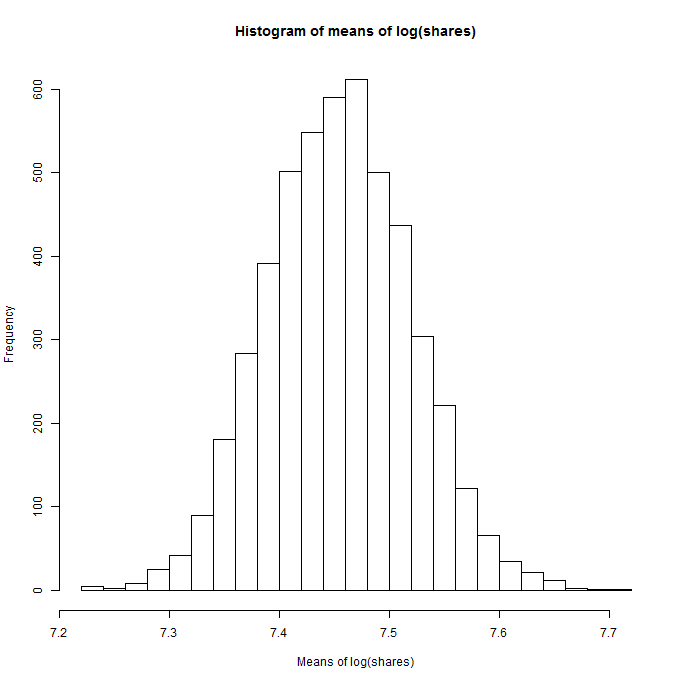
\includegraphics[width = 0.7\textwidth]{hist_means_of_log_shares.png}
   \caption{30-bin histogram of means of \texttt{$\log$(shares)}.}
   \label{img:hist_means_of_log_shares}
 \end{center}
\end{figure} 

\begin{table}
\caption{95\% confidence intervals (CI's) for mean of \texttt{$\log$(shares)}} \label{tbl:log_shares_stats}
\begin{center}
\begin{tabular}{|c|c|} 
 \hline
Mean & 7.45 \\ \hline 
Statistic CI & (5.94; 8.97) \\ \hline
Pivotal CI & (7.35; 7.56) \\ \hline
Nonpivotal CI & (7.33; 7.58) \\ \hline
\end{tabular}
\end{center}
\end{table}

\subsection*{Bootstraping the mode and the median}
The more the distribution resembles the  power law distribution, the more appropriate is to choose median of the distribution as the center value. That is because the median is very stable against outliers. 
And pivotal or non-pivotal bootstrap methods can be applied to medians. 

In case of mode it is hard to decide when the  bootstrap technique is appropriate. The mode, in some sense, is not a smooth functional of the distribution. So the result will be most likely uninterpretable. 

The \texttt{$\log$(shares)} is approximately distributed  normally, so the values of mean, median and mode are close to each other. Therefore in this case bootstrap  is likely to be a reliable method for computing confidence intervals of median and mode.   

Histograms of sample medians and modes are presented in Figure \ref{img:hist_medians_modes_log_shares}, and respective confidence intervals are presented in Table \ref{tbl:log_shares_and_shares_median_mode_CIs}. The distribution of the modes is far from the normal random variable  distribution, so pivotal confidence interval could be uncorrect. From the Table \ref{tbl:log_shares_and_shares_median_mode_CIs}, as one could notice, it is evident that value of the mode is close to the left border of non-pivotal confidence interval.   

\begin{figure}[h]
\begin{minipage}[h]{0.49\linewidth}
\center{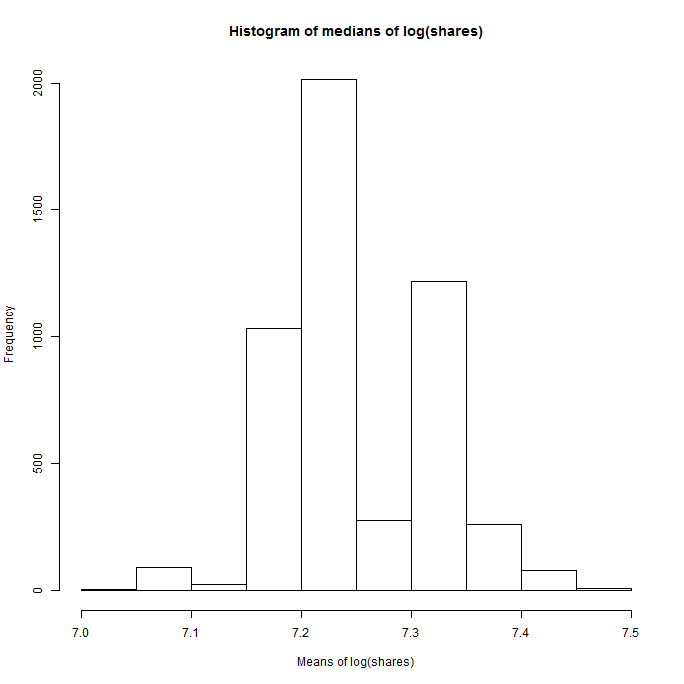
\includegraphics[width=0.95\linewidth]{hist_medians_of_log_shares.png} \\ a)}
\end{minipage}
\hfill
\begin{minipage}[h]{0.49\linewidth}
\center{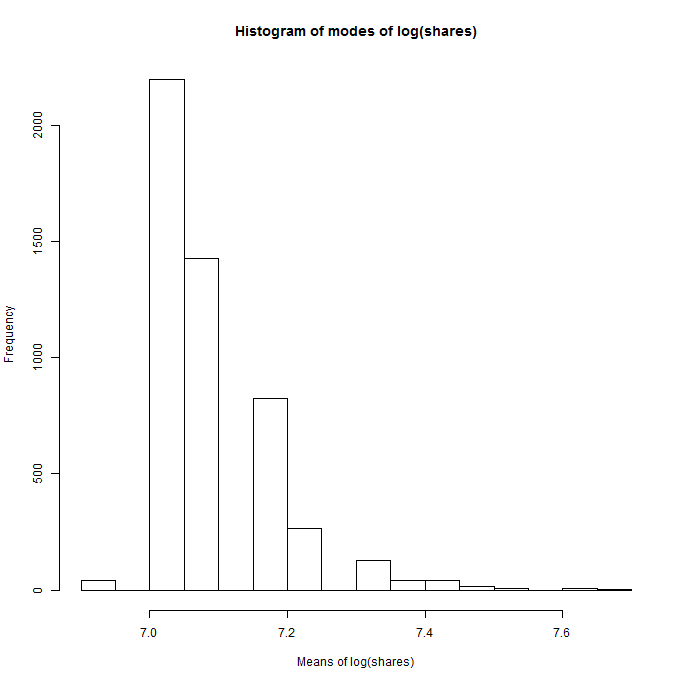
\includegraphics[width=0.95\linewidth]{hist_modes_of_log_shares.png} \\ b)}
\end{minipage}
\caption{Histograms of medians (a) and modes (b) of \texttt{$\log$(shares)}.}
\label{img:hist_medians_modes_log_shares}
\end{figure}

It is much more interesting to compute the confidence interval for median on initial scale, that is not  the median of logarithmic feature, but  the median of initial \texttt{shares} feature. Since the distribution of \texttt{shares} is more similar  to the power type distribution than to the normal one, it is better to choose the median as the central value due to the properties of median that were explained above.
In fact, we can use either pivotal or non-pivotal approaches to estimate a median because of the next theorem.

\begin{theorem}[Median Theorem, \cite{median_sample}]
Let a sample of size $n = 2m + 1$ with $n$ large be taken from an infinite population with a density
function $f(\bar{x})$ that is nonzero at the population median $\tilde{\mu}$ and continuously differentiable in a neighborhood of $\tilde{\mu}$. The sampling distribution of the median is approximately normal with mean $tilde{\mu}$ and variance $\frac{1}{8f(\tilde{\mu})^2 m}$.
\end{theorem}

The histogram of  sample medians  of \texttt{shares}  is presented at Figure \ref{img:hist_medians_modes_shares} (a), and computed confidence intervals are shown in the  Table  \ref{tbl:log_shares_and_shares_median_mode_CIs}. The mode's distribution is obviously far from normal (so we don't examine pivotal CI), and, as well as in the case of \texttt{$\log$(shares)} modes, the value of population mode is close to the left border of non-pivotal confidence interval. 

\begin{figure}[h]
\begin{minipage}[h]{0.49\linewidth}
\center{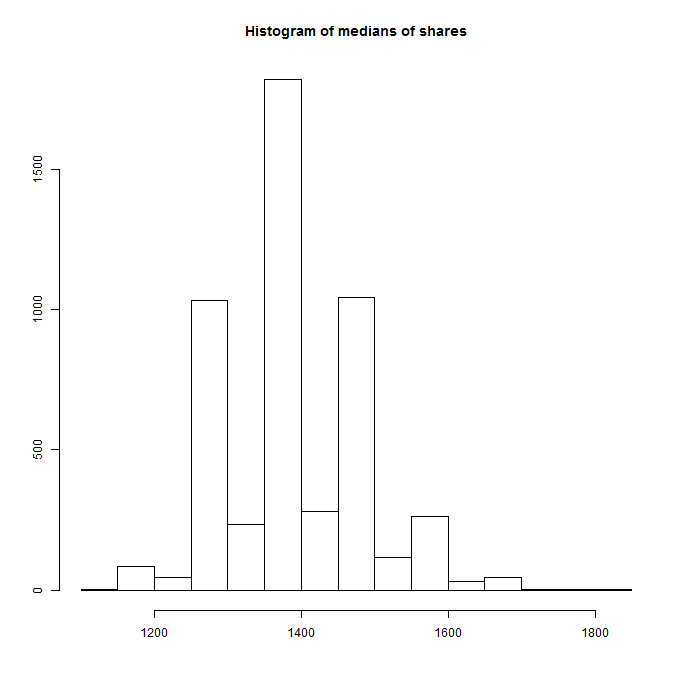
\includegraphics[width=0.95\linewidth]{hist_medians_of_shares.png} \\ a)}
\end{minipage}
\hfill
\begin{minipage}[h]{0.49\linewidth}
\center{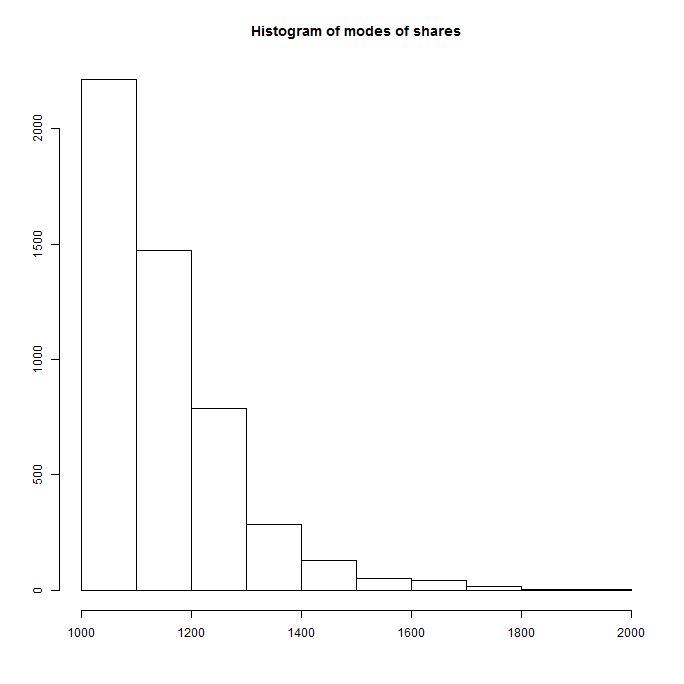
\includegraphics[width=0.95\linewidth]{hist_modes_of_shares.png} \\ b)}
\end{minipage}
\caption{Histograms of sample medians (a) and sample modes (b) of \texttt{shares}.}
\label{img:hist_medians_modes_shares}
\end{figure}

\begin{table}
\caption{95\% confidence intervals (CI's) for median and mode of \texttt{$\log$(shares)} and of \texttt{shares}} \label{tbl:log_shares_and_shares_median_mode_CIs}
\begin{center}
\begin{tabular}{|c|c|c||c|c|} 
 \hline
 & \multicolumn{2}{|c||}{\texttt{$\log$(shares)}} & \multicolumn{2}{|c|}{\texttt{shares}} \\ \hline 
& Median & Mode & Median & Mode  \\ \hline 
Value & 7.24 & 7.0 & 1400 & 1100 \\ \hline
Pivotal CI & (7.14; 7.36) & --- & (1257.76; 1571.5) & ---\\ \hline %(6.9; 7.26) (990.56; 1410.12) -- pivotals for modes
Nonpivotal CI & (7.17; 7.38) & (7.0; 7.3) & (1250; 1600) & (1100; 1500) \\ \hline
\end{tabular}
\end{center}
\end{table}  

\subsection*{Partitioning the population into two groups}
We split our \texttt{$\log$(shares)}  data according to the day, when the article was firstly published: workday or weekend. In our dataset we have seven dummy variables, indicating the day of publishing a news: \texttt{weekday\_is\_monday}, \texttt{weekday\_is\_tuesday}, \texttt{weekday\_is\_wed\-nes\-day}, \texttt{weekday\_is\_thursday}, \texttt{weekday\_is\_friday}, \texttt{weekday\_is\_saturday}, \texttt{weekday\_is\_sun\-day}. If we take entities, for which \texttt{weekday\_is\_saturday} or \texttt{weekday\_is\_sunday} are equal to 1, we will end up with the class \texttt{published\_on\_weekend}. All of the other entities will be considered as belonging to the class \texttt{published\_on\_workday}.  

Histograms of the sample means in each of the classes are shown in figure \ref{img:hist_log_shares_worday_weekend}. Each of the histrograms closely resembles the density of normal distribution, therefore pivotal and non-pivotal bootstrap methods should compute the similar confidence intervals (CI's). 95\% intervals for mean in each of the two groups are presented in Table \ref{tbl:workday_weekend_log_shares_CIs}.  

\begin{figure}[h!]
 \begin{center}
    \center 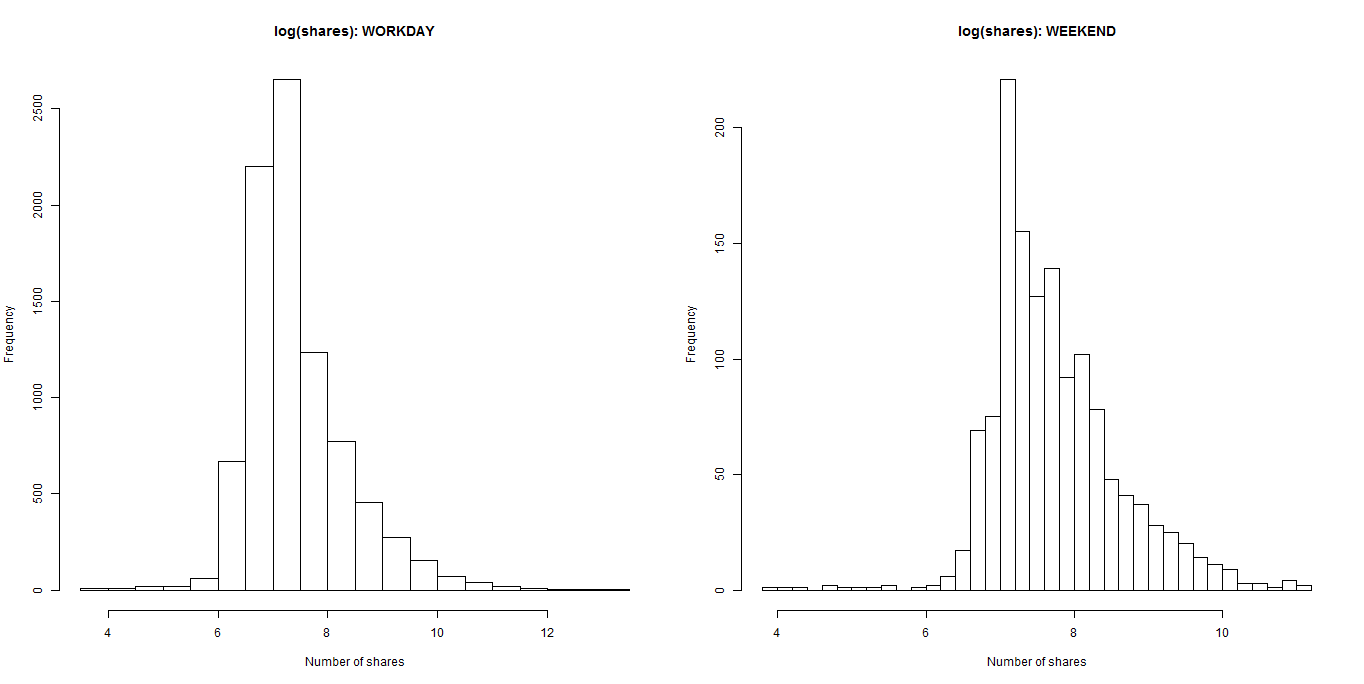
\includegraphics[width = 0.9\textwidth]{hist_log_shares_worday_weekend.png}
   \caption{30-bin histograms of \texttt{$\log$(shares)}, grouped by the day, when the article was published: workday (left) or weekend (right)}
   \label{img:hist_log_shares_worday_weekend}
 \end{center}
\end{figure} 

\begin{table}
\caption{Confidence intervals of mean of \texttt{$\log$(shares)} feature, grouped by a day, when the article was publishead: workday or weekend} \label{tbl:workday_weekend_log_shares_CIs}
\begin{center}
\begin{tabular}{|c|c|c|c|c|} 
 \hline
 & Workday & Weekend \\ \hline
Number of variables &  8660 & 1340 \\ \hline
Mean & 7.41 & 7.73 \\ \hline
Pivotal CI & (7.3; 7.5) & (7.63; 7.83)\\ \hline
Non-pivotal CI & (7.28; 7.54) & (7.6; 7.85)\\ \hline 
\end{tabular}
\end{center}
\end{table}

The CI of the mean in both classes do not intersect with each other, so we can claim with 95\% confidence that two means in these groups  are different.
 %But this is not a correct procedure, because ranges of means in workday and weekend articles groops intersected. 